\section{Markov Modelleri}
Markov modelleri, Markov zinciri adı verilen ve gelecekteki durumun yalnızca mevcut duruma bağlı olduğu bir süreç modellemesi türünü temsil eder. Bu model, geçmiş durumların gelecekteki durumları belirlemede tam olarak yeterli olduğunu varsayar. Bu, bir durumun gelecekteki olasılığını, yalnızca mevcut durumun bilgisine dayanarak tahmin etmek için kullanılır. Markov zincirleri, durumları temsil eden bir durum uzayı ve durumlar arasındaki geçiş olasılıklarını tanımlayan bir geçiş matrisi kullanır. Her bir durum, bir durum uzayının bir noktasını temsil eder ve geçiş matrisi, her bir durumun diğer durumlara geçiş olasılıklarını belirtir. Türleri:
\begin{itemize}
    \item Birinci Dereceden Markov Zinciri
    \item Yüksek Dereceden Markov Zinciri
    \item Gizli Markov Modeli (Hidden Markov Model - HMM)
\end{itemize}

\begin{figure}[h]
    \centering
    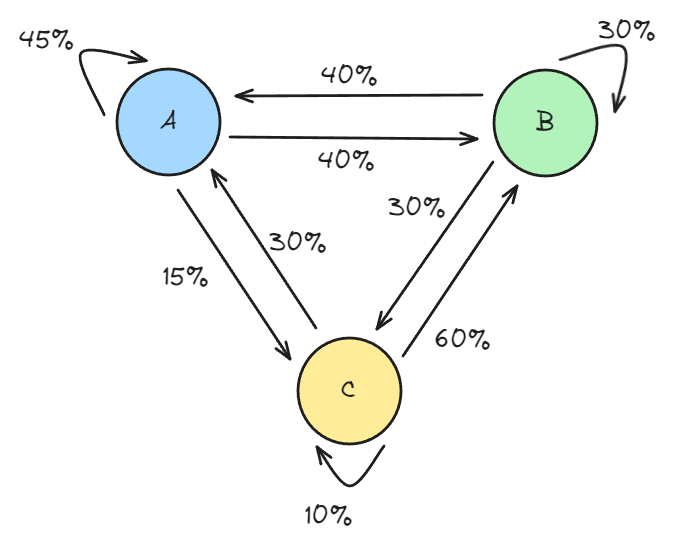
\includegraphics[width=1\textwidth]{images/markov_chains.png}
    \caption{Markov zinciri.}
    \label{fig:enter-label}
\end{figure}

\subsection{Birinci Dereceden Markov Zinciri}
Gelecekteki durum, yalnızca mevcut duruma bağlıdır. Bir sonraki durum, yalnızca mevcut durumun bilgisine dayanarak tahmin edilir.

\subsubsection{Çalışma Adımları}
\begin{enumerate}
    \item Modelin kullanılacağı durumlar tanımlanır.
    \item Her bir durumun, bir sonraki duruma geçme olasılığı belirlenir.
    \item Modelin başlangıç durumu (başlangıç noktası) seçilir.
    \item Başlangıç durumundan başlayarak, her bir adımda geçiş olasılıklarına dayanarak bir sonraki durum rastgele seçilir.
    \item Zincir belirlenen adımlar boyunca çalıştırılır ve bir sonraki durum tahmin edilir.
\end{enumerate}

\[P(X_{n+1} = s_j | X_n = s_i) = P_{ij}\]

\begin{itemize}
    \item $P_{ij}$, geçiş olasılığını ifade eden bir olasılık matrisinin elemanıdır.
    \item $P(X_{n+1} = s_j | X_n = s_i)$, durum  $s_{i}$'den durum $s_{j}$'ye geçişin olasığıdır.
\end{itemize}

\subsubsection{Python Kodu}

\begin{lstlisting}[language=Python]
import markovify

# Ornek metin
text = """
This is a sample text. This text will be analysed with a first order Markov chain. 
Markov chains are used to predict the next state based on the past state.
"""

# Markov zinciri modelini olusturma
model = markovify.Text(text, state_size=1)

# Rastgele bir dizi olusturma
generated_sequence = model.make_sentence()

print("Generated Sequence:", generated_sequence)
# Generated Sequence: This is a first order Markov chain.   
\end{lstlisting}

\subsection{Yüksek Dereceden Markov Zinciri}
Yüksek dereceden Markov zinciri, birinci derecede Markov zincirinden farklı olarak, daha önceki birden fazla durumu dikkate alarak bir sonraki durumu tahmin etmek için kullanılır. Geçmişteki birden fazla durumun etkilerini içeren daha karmaşık ilişkileri modelleyebilir. 

\[P(X_{n+1} = s_j | X_n = s_i, X_{n-1} = s_k, ..., X_{n-d} = s_l) = P_{ijkl...l}\]

\subsubsection{Python Kodu}

\begin{lstlisting}[language=Python]
import markovify

# Ornek metin
text = """
This is a sample text. This text will be analysed with a first order Markov chain. 
Markov chains are used to predict the next state based on the past state.
"""

# Markov zinciri modelini olusturma
model = markovify.Text(text, state_size=3)

# Rastgele bir dizi olusturma
generated_sequence = model.make_sentence()

print("Generated Sequence:", generated_sequence)
# Generated Sequence: This is a first order Markov chain.   
\end{lstlisting}

\subsection{Hidden Markov Model (HMM)}
Zamanla değişen gizli durumların gözlemlenebilir durumlar aracılığıyla modellendiği bir olasılıksal modeldir. HMM, bir Markov zincirinin gizli bir durumla eşlenmesiyle oluşturulur ve bu gizli durumlar gözlemlenebilir durumlarla ilişkilendirilir. İki tür durumu içerir:
\begin{itemize}
    \item \textbf{Gizli Durumlar (Hidden States):} Gözlemleyiciler tarafından doğrudan gözlemlenemeyen ve model tarafından tahmin edilmeye çalışılan durumlardır. 
    \item \textbf{Gözlemlenebilir Durumlar (Observable States):} Model tarafından gözlemlenebilen durumlardır. Bu durumlar gizli durumlarla ilişkilendirilir ve belirli bir zaman aralığında gözlenen gerçek verilerdir.
\end{itemize}

\subsubsection{Çalışma Adımları}
\begin{itemize}
    \item Modelin kullanacağı gizli ve gözlemlenebilir durumlar tanımlanır.
    \item Gizli durumlar arasındaki geçiş olasılıkları belirlenir.
    \item Her bir gizli durumun gözlemlenebilir durumlarla ilişkilendirilme olasılıkları belirlenir.
    \item Modelin başlangıç durumu belirlenir.
    \item Model genellikle gözlemlenen veriler kullanılarak eğitilir. Bu, Viterbi algoritması veya Baum-Welch algoritması gibi yöntemler kullanılarak gerçekleştirilebilir.
\end{itemize}

\[P(Y_1=y_1, Y_2=y_2, ..., Y_n=y_n, X_1=x_1, X_2=x_2, ..., X_n=x_n) = P(X_1) \cdot P(Y_1|X_1) \cdot \prod_{t=2}^{n} P(X_t|X_{t-1}) \cdot P(Y_t|X_t)\]
\begin{itemize}
    \item $Y_{n}$, gözlemlenebilir durumları
    \item $X_{n}$, gizli durumları
    \item $P(X_1)$, başlangıç durumunun olasılığını
    \item $P(Y_{t} | X_{t})$, gözlemlenebilir durumların gizli durumlar altında koşulluk olasılıklarını
    \item $P(X_{t} | X_{t-1})$, gizli durumların birbirine geçiş olasılıklarını
\end{itemize}

\subsubsection{Python Kodu}

\begin{lstlisting}[language=Python]
from hmmlearn import hmm
import numpy as np

# Ornek veri
X = np.array([[0], [1], [0], [1], [0], [1], [0], [1]])
lengths = [8]  # Gozlemlenen verinin uzunlugu

# Gizli Markov Modeli olusturma
model = hmm.GaussianHMM(n_components=2, covariance_type="full")

# Modeli egitme
model.fit(X, lengths)

# Gizli durumlari tahmin etme
predicted_states = model.predict(X)

print("Gizli Durumlar:", predicted_states)
\end{lstlisting}

\newpage